% Created by tikzDevice version 0.12.3.1 on 2021-05-03 23:03:22
% !TEX encoding = UTF-8 Unicode
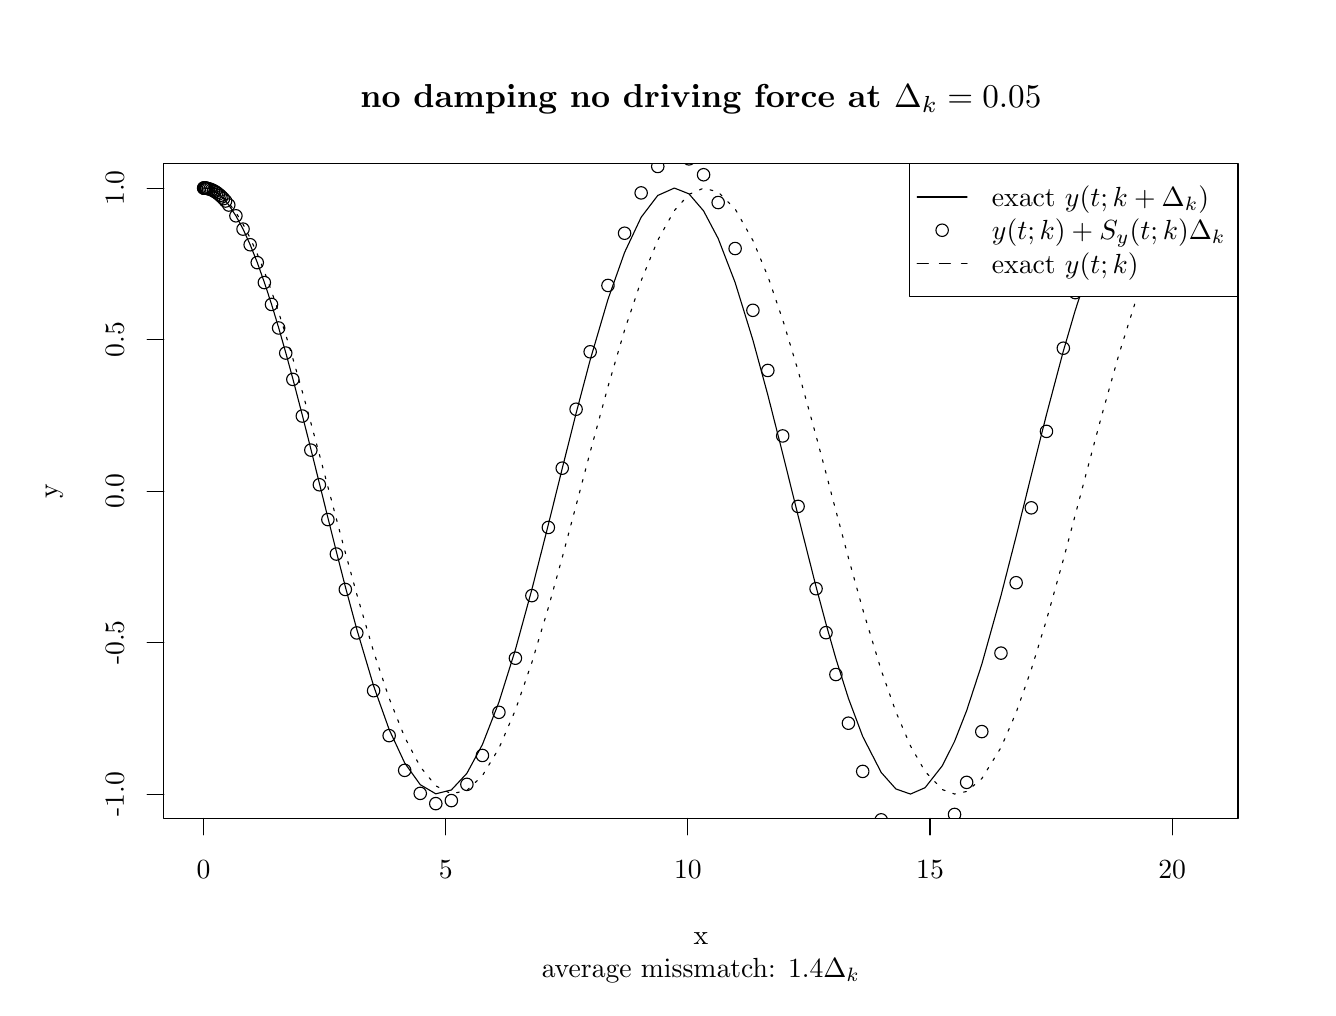
\begin{tikzpicture}[x=1pt,y=1pt]
\definecolor{fillColor}{RGB}{255,255,255}
\path[use as bounding box,fill=fillColor,fill opacity=0.00] (0,0) rectangle (462.53,346.90);
\begin{scope}
\path[clip] ( 49.20, 61.20) rectangle (437.33,297.70);
\definecolor{drawColor}{RGB}{0,0,0}

\path[draw=drawColor,line width= 0.4pt,line join=round,line cap=round] ( 63.58,288.94) --
	( 63.67,288.94) --
	( 63.79,288.93) --
	( 63.91,288.93) --
	( 64.03,288.92) --
	( 64.16,288.91) --
	( 64.28,288.90) --
	( 64.40,288.89) --
	( 64.57,288.86) --
	( 64.84,288.82) --
	( 65.30,288.71) --
	( 65.91,288.53) --
	( 66.51,288.29) --
	( 67.12,288.00) --
	( 67.72,287.66) --
	( 68.33,287.25) --
	( 68.93,286.80) --
	( 69.54,286.29) --
	( 70.14,285.73) --
	( 70.75,285.12) --
	( 71.51,284.27) --
	( 72.67,282.82) --
	( 75.25,278.91) --
	( 77.82,274.13) --
	( 80.39,268.48) --
	( 82.96,262.04) --
	( 85.53,254.85) --
	( 88.11,246.98) --
	( 90.68,238.50) --
	( 93.25,229.48) --
	( 95.82,220.02) --
	( 99.24,206.87) --
	(102.32,194.67) --
	(105.40,182.27) --
	(108.48,169.84) --
	(111.55,157.53) --
	(114.78,144.91) --
	(118.93,129.48) --
	(125.00,109.06) --
	(130.62, 93.29) --
	(136.23, 81.21) --
	(141.85, 73.36) --
	(147.47, 70.05) --
	(153.09, 71.44) --
	(158.71, 77.46) --
	(164.32, 87.86) --
	(170.28,103.17) --
	(176.24,122.16) --
	(182.19,143.91) --
	(188.15,167.37) --
	(193.16,187.60) --
	(198.17,207.55) --
	(203.25,226.80) --
	(209.69,248.73) --
	(215.69,265.67) --
	(221.68,278.39) --
	(227.68,286.27) --
	(233.68,288.94) --
	(238.95,286.85) --
	(244.23,280.70) --
	(249.51,270.71) --
	(255.64,254.80) --
	(262.06,234.01) --
	(267.45,214.18) --
	(272.83,192.97) --
	(278.39,170.55) --
	(284.88,144.90) --
	(288.47,131.47) --
	(292.05,118.88) --
	(296.58,104.54) --
	(301.74, 90.78) --
	(308.42, 77.77) --
	(313.71, 71.82) --
	(318.99, 69.96) --
	(324.28, 72.27) --
	(330.54, 80.24) --
	(334.92, 88.99) --
	(339.29,100.10) --
	(344.77,116.87) --
	(351.70,141.67) --
	(357.18,163.11) --
	(362.66,185.21) --
	(368.14,207.09) --
	(374.23,230.02) --
	(378.54,244.78) --
	(382.85,257.88) --
	(387.95,270.79) --
	(394.40,282.47) --
	(400.26,288.03) --
	(406.12,288.52) --
	(411.97,283.93) --
	(417.83,274.47) --
	(422.95,262.54);
\end{scope}
\begin{scope}
\path[clip] (  0.00,  0.00) rectangle (462.53,346.90);
\definecolor{drawColor}{RGB}{0,0,0}

\path[draw=drawColor,line width= 0.4pt,line join=round,line cap=round] ( 63.58, 61.20) -- (413.56, 61.20);

\path[draw=drawColor,line width= 0.4pt,line join=round,line cap=round] ( 63.58, 61.20) -- ( 63.58, 55.20);

\path[draw=drawColor,line width= 0.4pt,line join=round,line cap=round] (151.07, 61.20) -- (151.07, 55.20);

\path[draw=drawColor,line width= 0.4pt,line join=round,line cap=round] (238.57, 61.20) -- (238.57, 55.20);

\path[draw=drawColor,line width= 0.4pt,line join=round,line cap=round] (326.07, 61.20) -- (326.07, 55.20);

\path[draw=drawColor,line width= 0.4pt,line join=round,line cap=round] (413.56, 61.20) -- (413.56, 55.20);

\node[text=drawColor,anchor=base,inner sep=0pt, outer sep=0pt, scale=  1.00] at ( 63.58, 39.60) {0};

\node[text=drawColor,anchor=base,inner sep=0pt, outer sep=0pt, scale=  1.00] at (151.07, 39.60) {5};

\node[text=drawColor,anchor=base,inner sep=0pt, outer sep=0pt, scale=  1.00] at (238.57, 39.60) {10};

\node[text=drawColor,anchor=base,inner sep=0pt, outer sep=0pt, scale=  1.00] at (326.07, 39.60) {15};

\node[text=drawColor,anchor=base,inner sep=0pt, outer sep=0pt, scale=  1.00] at (413.56, 39.60) {20};

\path[draw=drawColor,line width= 0.4pt,line join=round,line cap=round] ( 49.20, 69.95) -- ( 49.20,288.94);

\path[draw=drawColor,line width= 0.4pt,line join=round,line cap=round] ( 49.20, 69.95) -- ( 43.20, 69.95);

\path[draw=drawColor,line width= 0.4pt,line join=round,line cap=round] ( 49.20,124.70) -- ( 43.20,124.70);

\path[draw=drawColor,line width= 0.4pt,line join=round,line cap=round] ( 49.20,179.44) -- ( 43.20,179.44);

\path[draw=drawColor,line width= 0.4pt,line join=round,line cap=round] ( 49.20,234.19) -- ( 43.20,234.19);

\path[draw=drawColor,line width= 0.4pt,line join=round,line cap=round] ( 49.20,288.94) -- ( 43.20,288.94);

\node[text=drawColor,rotate= 90.00,anchor=base,inner sep=0pt, outer sep=0pt, scale=  1.00] at ( 34.80, 69.95) {-1.0};

\node[text=drawColor,rotate= 90.00,anchor=base,inner sep=0pt, outer sep=0pt, scale=  1.00] at ( 34.80,124.70) {-0.5};

\node[text=drawColor,rotate= 90.00,anchor=base,inner sep=0pt, outer sep=0pt, scale=  1.00] at ( 34.80,179.44) {0.0};

\node[text=drawColor,rotate= 90.00,anchor=base,inner sep=0pt, outer sep=0pt, scale=  1.00] at ( 34.80,234.19) {0.5};

\node[text=drawColor,rotate= 90.00,anchor=base,inner sep=0pt, outer sep=0pt, scale=  1.00] at ( 34.80,288.94) {1.0};

\path[draw=drawColor,line width= 0.4pt,line join=round,line cap=round] ( 49.20, 61.20) --
	(437.33, 61.20) --
	(437.33,297.70) --
	( 49.20,297.70) --
	( 49.20, 61.20);
\end{scope}
\begin{scope}
\path[clip] (  0.00,  0.00) rectangle (462.53,346.90);
\definecolor{drawColor}{RGB}{0,0,0}

\node[text=drawColor,anchor=base,inner sep=0pt, outer sep=0pt, scale=  1.20] at (243.26,318.16) {\bfseries  no damping no driving force at $\Delta_k = 0.05$};

\node[text=drawColor,anchor=base,inner sep=0pt, outer sep=0pt, scale=  1.00] at (243.26,  3.60) {average missmatch: $1.4 \Delta_k$};

\node[text=drawColor,anchor=base,inner sep=0pt, outer sep=0pt, scale=  1.00] at (243.26, 15.60) {x};

\node[text=drawColor,rotate= 90.00,anchor=base,inner sep=0pt, outer sep=0pt, scale=  1.00] at ( 10.80,179.45) {y};
\end{scope}
\begin{scope}
\path[clip] ( 49.20, 61.20) rectangle (437.33,297.70);
\definecolor{drawColor}{RGB}{0,0,0}

\path[draw=drawColor,line width= 0.4pt,line join=round,line cap=round] ( 63.58,288.94) circle (  2.25);

\path[draw=drawColor,line width= 0.4pt,line join=round,line cap=round] ( 63.67,288.94) circle (  2.25);

\path[draw=drawColor,line width= 0.4pt,line join=round,line cap=round] ( 63.79,288.93) circle (  2.25);

\path[draw=drawColor,line width= 0.4pt,line join=round,line cap=round] ( 63.91,288.93) circle (  2.25);

\path[draw=drawColor,line width= 0.4pt,line join=round,line cap=round] ( 64.03,288.92) circle (  2.25);

\path[draw=drawColor,line width= 0.4pt,line join=round,line cap=round] ( 64.16,288.91) circle (  2.25);

\path[draw=drawColor,line width= 0.4pt,line join=round,line cap=round] ( 64.28,288.89) circle (  2.25);

\path[draw=drawColor,line width= 0.4pt,line join=round,line cap=round] ( 64.40,288.88) circle (  2.25);

\path[draw=drawColor,line width= 0.4pt,line join=round,line cap=round] ( 64.57,288.86) circle (  2.25);

\path[draw=drawColor,line width= 0.4pt,line join=round,line cap=round] ( 64.84,288.81) circle (  2.25);

\path[draw=drawColor,line width= 0.4pt,line join=round,line cap=round] ( 65.30,288.71) circle (  2.25);

\path[draw=drawColor,line width= 0.4pt,line join=round,line cap=round] ( 65.91,288.53) circle (  2.25);

\path[draw=drawColor,line width= 0.4pt,line join=round,line cap=round] ( 66.51,288.29) circle (  2.25);

\path[draw=drawColor,line width= 0.4pt,line join=round,line cap=round] ( 67.12,288.00) circle (  2.25);

\path[draw=drawColor,line width= 0.4pt,line join=round,line cap=round] ( 67.72,287.65) circle (  2.25);

\path[draw=drawColor,line width= 0.4pt,line join=round,line cap=round] ( 68.33,287.25) circle (  2.25);

\path[draw=drawColor,line width= 0.4pt,line join=round,line cap=round] ( 68.93,286.79) circle (  2.25);

\path[draw=drawColor,line width= 0.4pt,line join=round,line cap=round] ( 69.54,286.29) circle (  2.25);

\path[draw=drawColor,line width= 0.4pt,line join=round,line cap=round] ( 70.14,285.72) circle (  2.25);

\path[draw=drawColor,line width= 0.4pt,line join=round,line cap=round] ( 70.75,285.11) circle (  2.25);

\path[draw=drawColor,line width= 0.4pt,line join=round,line cap=round] ( 71.51,284.26) circle (  2.25);

\path[draw=drawColor,line width= 0.4pt,line join=round,line cap=round] ( 72.67,282.81) circle (  2.25);

\path[draw=drawColor,line width= 0.4pt,line join=round,line cap=round] ( 75.25,278.91) circle (  2.25);

\path[draw=drawColor,line width= 0.4pt,line join=round,line cap=round] ( 77.82,274.11) circle (  2.25);

\path[draw=drawColor,line width= 0.4pt,line join=round,line cap=round] ( 80.39,268.46) circle (  2.25);

\path[draw=drawColor,line width= 0.4pt,line join=round,line cap=round] ( 82.96,262.00) circle (  2.25);

\path[draw=drawColor,line width= 0.4pt,line join=round,line cap=round] ( 85.53,254.79) circle (  2.25);

\path[draw=drawColor,line width= 0.4pt,line join=round,line cap=round] ( 88.11,246.89) circle (  2.25);

\path[draw=drawColor,line width= 0.4pt,line join=round,line cap=round] ( 90.68,238.38) circle (  2.25);

\path[draw=drawColor,line width= 0.4pt,line join=round,line cap=round] ( 93.25,229.32) circle (  2.25);

\path[draw=drawColor,line width= 0.4pt,line join=round,line cap=round] ( 95.82,219.80) circle (  2.25);

\path[draw=drawColor,line width= 0.4pt,line join=round,line cap=round] ( 99.24,206.56) circle (  2.25);

\path[draw=drawColor,line width= 0.4pt,line join=round,line cap=round] (102.32,194.25) circle (  2.25);

\path[draw=drawColor,line width= 0.4pt,line join=round,line cap=round] (105.40,181.73) circle (  2.25);

\path[draw=drawColor,line width= 0.4pt,line join=round,line cap=round] (108.48,169.16) circle (  2.25);

\path[draw=drawColor,line width= 0.4pt,line join=round,line cap=round] (111.55,156.69) circle (  2.25);

\path[draw=drawColor,line width= 0.4pt,line join=round,line cap=round] (114.78,143.89) circle (  2.25);

\path[draw=drawColor,line width= 0.4pt,line join=round,line cap=round] (118.93,128.19) circle (  2.25);

\path[draw=drawColor,line width= 0.4pt,line join=round,line cap=round] (125.00,107.32) circle (  2.25);

\path[draw=drawColor,line width= 0.4pt,line join=round,line cap=round] (130.62, 91.08) circle (  2.25);

\path[draw=drawColor,line width= 0.4pt,line join=round,line cap=round] (136.23, 78.53) circle (  2.25);

\path[draw=drawColor,line width= 0.4pt,line join=round,line cap=round] (141.85, 70.21) circle (  2.25);

\path[draw=drawColor,line width= 0.4pt,line join=round,line cap=round] (147.47, 66.51) circle (  2.25);

\path[draw=drawColor,line width= 0.4pt,line join=round,line cap=round] (153.09, 67.60) circle (  2.25);

\path[draw=drawColor,line width= 0.4pt,line join=round,line cap=round] (158.71, 73.47) circle (  2.25);

\path[draw=drawColor,line width= 0.4pt,line join=round,line cap=round] (164.32, 83.91) circle (  2.25);

\path[draw=drawColor,line width= 0.4pt,line join=round,line cap=round] (170.28, 99.50) circle (  2.25);

\path[draw=drawColor,line width= 0.4pt,line join=round,line cap=round] (176.24,119.06) circle (  2.25);

\path[draw=drawColor,line width= 0.4pt,line join=round,line cap=round] (182.19,141.67) circle (  2.25);

\path[draw=drawColor,line width= 0.4pt,line join=round,line cap=round] (188.15,166.30) circle (  2.25);

\path[draw=drawColor,line width= 0.4pt,line join=round,line cap=round] (193.16,187.72) circle (  2.25);

\path[draw=drawColor,line width= 0.4pt,line join=round,line cap=round] (198.17,209.02) circle (  2.25);

\path[draw=drawColor,line width= 0.4pt,line join=round,line cap=round] (203.25,229.78) circle (  2.25);

\path[draw=drawColor,line width= 0.4pt,line join=round,line cap=round] (209.69,253.75) circle (  2.25);

\path[draw=drawColor,line width= 0.4pt,line join=round,line cap=round] (215.69,272.62) circle (  2.25);

\path[draw=drawColor,line width= 0.4pt,line join=round,line cap=round] (221.68,287.19) circle (  2.25);

\path[draw=drawColor,line width= 0.4pt,line join=round,line cap=round] (227.68,296.74) circle (  2.25);

\path[draw=drawColor,line width= 0.4pt,line join=round,line cap=round] (233.68,300.74) circle (  2.25);

\path[draw=drawColor,line width= 0.4pt,line join=round,line cap=round] (238.95,299.49) circle (  2.25);

\path[draw=drawColor,line width= 0.4pt,line join=round,line cap=round] (244.23,293.75) circle (  2.25);

\path[draw=drawColor,line width= 0.4pt,line join=round,line cap=round] (249.51,283.71) circle (  2.25);

\path[draw=drawColor,line width= 0.4pt,line join=round,line cap=round] (255.64,267.09) circle (  2.25);

\path[draw=drawColor,line width= 0.4pt,line join=round,line cap=round] (262.06,244.77) circle (  2.25);

\path[draw=drawColor,line width= 0.4pt,line join=round,line cap=round] (267.45,223.03) circle (  2.25);

\path[draw=drawColor,line width= 0.4pt,line join=round,line cap=round] (272.83,199.37) circle (  2.25);

\path[draw=drawColor,line width= 0.4pt,line join=round,line cap=round] (278.39,173.91) circle (  2.25);

\path[draw=drawColor,line width= 0.4pt,line join=round,line cap=round] (284.88,144.17) circle (  2.25);

\path[draw=drawColor,line width= 0.4pt,line join=round,line cap=round] (288.47,128.28) circle (  2.25);

\path[draw=drawColor,line width= 0.4pt,line join=round,line cap=round] (292.05,113.16) circle (  2.25);

\path[draw=drawColor,line width= 0.4pt,line join=round,line cap=round] (296.58, 95.57) circle (  2.25);

\path[draw=drawColor,line width= 0.4pt,line join=round,line cap=round] (301.74, 78.15) circle (  2.25);

\path[draw=drawColor,line width= 0.4pt,line join=round,line cap=round] (308.42, 60.65) circle (  2.25);

\path[draw=drawColor,line width= 0.4pt,line join=round,line cap=round] (313.71, 51.54) circle (  2.25);

\path[draw=drawColor,line width= 0.4pt,line join=round,line cap=round] (318.99, 47.04) circle (  2.25);

\path[draw=drawColor,line width= 0.4pt,line join=round,line cap=round] (324.28, 47.36) circle (  2.25);

\path[draw=drawColor,line width= 0.4pt,line join=round,line cap=round] (330.54, 54.02) circle (  2.25);

\path[draw=drawColor,line width= 0.4pt,line join=round,line cap=round] (334.92, 62.60) circle (  2.25);

\path[draw=drawColor,line width= 0.4pt,line join=round,line cap=round] (339.29, 74.19) circle (  2.25);

\path[draw=drawColor,line width= 0.4pt,line join=round,line cap=round] (344.77, 92.54) circle (  2.25);

\path[draw=drawColor,line width= 0.4pt,line join=round,line cap=round] (351.70,120.89) circle (  2.25);

\path[draw=drawColor,line width= 0.4pt,line join=round,line cap=round] (357.18,146.33) circle (  2.25);

\path[draw=drawColor,line width= 0.4pt,line join=round,line cap=round] (362.66,173.39) circle (  2.25);

\path[draw=drawColor,line width= 0.4pt,line join=round,line cap=round] (368.14,201.02) circle (  2.25);

\path[draw=drawColor,line width= 0.4pt,line join=round,line cap=round] (374.23,231.07) circle (  2.25);

\path[draw=drawColor,line width= 0.4pt,line join=round,line cap=round] (378.54,251.16) circle (  2.25);

\path[draw=drawColor,line width= 0.4pt,line join=round,line cap=round] (382.85,269.70) circle (  2.25);

\path[draw=drawColor,line width= 0.4pt,line join=round,line cap=round] (387.95,289.02) circle (  2.25);

\path[draw=drawColor,line width= 0.4pt,line join=round,line cap=round] (394.40,308.40) circle (  2.25);

\path[draw=drawColor,line width= 0.4pt,line join=round,line cap=round] (400.26,320.23) circle (  2.25);

\path[draw=drawColor,line width= 0.4pt,line join=round,line cap=round] (406.12,325.94) circle (  2.25);

\path[draw=drawColor,line width= 0.4pt,line join=round,line cap=round] (411.97,325.21) circle (  2.25);

\path[draw=drawColor,line width= 0.4pt,line join=round,line cap=round] (417.83,317.99) circle (  2.25);

\path[draw=drawColor,line width= 0.4pt,line join=round,line cap=round] (422.95,306.53) circle (  2.25);

\path[draw=drawColor,line width= 0.4pt,dash pattern=on 1pt off 3pt ,line join=round,line cap=round] ( 63.58,288.94) --
	( 63.67,288.94) --
	( 63.79,288.93) --
	( 63.91,288.93) --
	( 64.03,288.92) --
	( 64.16,288.91) --
	( 64.28,288.90) --
	( 64.40,288.89) --
	( 64.57,288.87) --
	( 64.84,288.83) --
	( 65.30,288.74) --
	( 65.91,288.58) --
	( 66.51,288.37) --
	( 67.12,288.11) --
	( 67.72,287.81) --
	( 68.33,287.46) --
	( 68.93,287.06) --
	( 69.54,286.61) --
	( 70.14,286.11) --
	( 70.75,285.57) --
	( 71.51,284.82) --
	( 72.67,283.54) --
	( 75.25,280.10) --
	( 77.82,275.86) --
	( 80.39,270.86) --
	( 82.96,265.13) --
	( 85.53,258.73) --
	( 88.11,251.69) --
	( 90.68,244.08) --
	( 93.25,235.95) --
	( 95.82,227.38) --
	( 99.24,215.39) --
	(102.32,204.18) --
	(105.40,192.68) --
	(108.48,181.04) --
	(111.55,169.38) --
	(114.78,157.25) --
	(118.93,142.14) --
	(125.00,121.45) --
	(130.62,104.58) --
	(136.23, 90.54) --
	(141.85, 79.85) --
	(147.47, 72.93) --
	(153.09, 70.04) --
	(158.71, 71.28) --
	(164.32, 76.60) --
	(170.28, 86.49) --
	(176.24,100.33) --
	(182.19,117.52) --
	(188.15,137.35) --
	(193.16,155.45) --
	(198.17,174.26) --
	(203.25,193.50) --
	(209.69,217.19) --
	(215.69,237.59) --
	(221.68,255.48) --
	(227.68,270.10) --
	(233.68,280.82) --
	(238.95,286.65) --
	(244.23,288.91) --
	(249.51,287.52) --
	(255.64,281.38) --
	(262.06,270.03) --
	(267.45,257.05) --
	(272.83,241.36) --
	(278.39,222.94) --
	(284.88,199.44) --
	(288.47,185.93) --
	(292.05,172.32) --
	(296.58,155.33) --
	(301.74,136.74) --
	(308.42,114.74) --
	(313.71, 99.72) --
	(318.99, 87.38) --
	(324.28, 78.12) --
	(330.54, 71.57) --
	(334.92, 69.98) --
	(339.29, 70.90) --
	(344.77, 75.56) --
	(351.70, 86.76) --
	(357.18, 99.44) --
	(362.66,115.00) --
	(368.14,132.88) --
	(374.23,154.67) --
	(378.54,170.82) --
	(382.85,187.15) --
	(387.95,206.23) --
	(394.40,229.12) --
	(400.26,247.77) --
	(406.12,263.62) --
	(411.97,276.00) --
	(417.83,284.43) --
	(422.95,288.27);
\definecolor{fillColor}{RGB}{255,255,255}

\path[draw=drawColor,line width= 0.4pt,line join=round,line cap=round,fill=fillColor] (318.74,297.70) rectangle (437.33,249.70);

\path[draw=drawColor,line width= 0.4pt,line join=round,line cap=round] (321.44,285.70) -- (339.44,285.70);

\path[draw=drawColor,line width= 0.4pt,dash pattern=on 4pt off 4pt ,line join=round,line cap=round] (321.44,261.70) -- (339.44,261.70);

\path[draw=drawColor,line width= 0.4pt,line join=round,line cap=round] (330.44,273.70) circle (  2.25);

\node[text=drawColor,anchor=base west,inner sep=0pt, outer sep=0pt, scale=  1.00] at (348.44,282.25) {exact $y(t;k+\Delta_k)$};

\node[text=drawColor,anchor=base west,inner sep=0pt, outer sep=0pt, scale=  1.00] at (348.44,270.25) {$y(t;k) + S_y(t;k) \Delta_k$};

\node[text=drawColor,anchor=base west,inner sep=0pt, outer sep=0pt, scale=  1.00] at (348.44,258.25) {exact $y(t;k)$};
\end{scope}
\end{tikzpicture}
